\newpage
\section{Comparison}
\label{sec:verify}


The Table below compares the result to the state-of-the-art on three different benchmarks clustering accuracy (ACC), normalized mutual information (NMI), and adjusted rand index (ARI). 


%
%\begin{figure}[!htbp]
%\begin{center}
%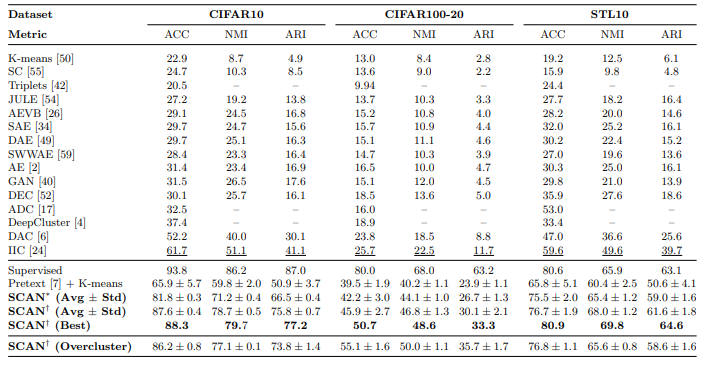
\includegraphics[width=6in]{3.PNG}
%\end{center}
%\caption{ \label{fig:first}}
%\end{figure}
%
%

%%% STATE-OF-THE-ART TABLE %%%%
\setlength{\tabcolsep}{4pt}
\begin{table}[ht]
\begin{center}
\label{table:sota}
\resizebox{\columnwidth}{!}{
\begin{tabular}{@{}l c ccc c ccc c ccc@{}}
\toprule
\textbf{Dataset} && \multicolumn{3}{c}{\textbf{CIFAR10}} && \multicolumn{3}{c}{\textbf{CIFAR100-20}} && \multicolumn{3}{c}{\textbf{STL10}} \\
\cmidrule{3-5} \cmidrule{7-9} \cmidrule{11-13}
\textbf{Metric} && ACC & NMI & ARI && ACC & NMI & ARI&& ACC & NMI & ARI \\
\midrule
\noalign{\smallskip}

K-means~\cite{wang2015optimized}     && 22.9 & 8.7   & 4.9  && 13.0  & 8.4  & 2.8 && 19.2 & 12.5 & 6.1  \\
Triplets~\cite{schultz2004learning}  && 20.5 & --    & --   && 9.94  & --   & --  && 24.4 & --   & --   \\
JULE~\cite{yang2016joint}            && 27.2 & 19.2  & 13.8 && 13.7  & 10.3 & 3.3 && 27.7 & 18.2 & 16.4 \\
AEVB~\cite{kingma2013auto}           && 29.1 & 24.5  & 16.8 && 15.2  & 10.8 & 4.0 && 28.2 & 20.0 & 14.6 \\
SAE~\cite{ng2011sparse}              && 29.7 & 24.7  & 15.6 && 15.7  & 10.9 & 4.4 && 32.0 & 25.2 & 16.1 \\
DAE~\cite{vincent2010stacked}        && 29.7 & 25.1  & 16.3 && 15.1  & 11.1 & 4.6 && 30.2 & 22.4 & 15.2 \\
SWWAE~\cite{zhao2015stacked}         && 28.4 & 23.3  & 16.4 && 14.7  & 10.3 & 3.9 && 27.0 & 19.6 & 13.6 \\
AE~\cite{bengio2007greedy}           && 31.4 & 23.4  & 16.9 && 16.5  & 10.0 & 4.7 && 30.3 & 25.0 & 16.1 \\
GAN~\cite{radford2015unsupervised}   && 31.5 & 26.5  & 17.6 && 15.1  & 12.0 & 4.5 && 29.8 & 21.0 & 13.9 \\
DEC~\cite{DEC}                       && 30.1 & 25.7  & 16.1 && 18.5  & 13.6 & 5.0 && 35.9 & 27.6 & 18.6 \\
ADC~\cite{haeusser2018associative}   && 32.5 & --    & --   && 16.0  & --   & --  && 53.0 & --   & --   \\
DeepCluster~\cite{DeepCluster}       && 37.4 & --    & --   && 18.9  & --   & --  && 33.4 & --   & --   \\
DAC~\cite{DAC}                       && 52.2 & 40.0 & 30.1 && 23.8& 18.5 & 8.8 && 47.0 & 36.6 & 25.6 \\
IIC~\cite{IIC} && \underline{61.7} & \underline{51.1}  & \underline{41.1} && \underline{25.7}  & \underline{22.5} & \underline{11.7}&& \underline{59.6} & \underline{49.6} & \underline{39.7} \\
%\textbf{SCAN$^\dagger$ (Ours)} && \textbf{88.6} & \textbf{80.3} & \textbf{77.9} && \textbf{50.5} & \textbf{47.4} & \textbf{32.8} && \textbf{81.2} & \textbf{70.1} & \textbf{65.1} \\
\midrule
Supervised  && 93.8 &  86.2 & 87.0   && 80.0 & 68.0 & 63.2 && 80.6 & 65.9 & 63.1\\
Pretext~\cite{chen2020simple} + K-means && $65.9\pm5.7$ & $59.8\pm2.0$ & $50.9\pm3.7$   && $39.5\pm1.9$ & $40.2\pm1.1$ & $23.9\pm1.1$ && $65.8\pm5.1$ & $60.4\pm2.5$ & $50.6\pm4.1$\\
\textbf{SCAN$^*$ (Avg $\pm$ Std) }  &&$81.8\pm0.3$ & $71.2\pm 0.4$ & $66.5\pm0.4 $&& $42.2\pm3.0$ & $44.1\pm1.0$ & $26.7\pm1.3$ && $75.5\pm2.0$ & $65.4\pm1.2$&$59.0\pm1.6$  \\
\textbf{SCAN$^\dagger$ (Avg $\pm$ Std) } &&$87.6\pm0.4$ & $78.7\pm 0.5$ & $75.8\pm0.7 $&& $45.9\pm2.7$ & $46.8\pm1.3$ & $30.1\pm2.1$ && $76.7\pm1.9$ & $68.0\pm1.2$&$61.6\pm1.8$  \\
\textbf{SCAN$^\dagger$ (Best)} && \textbf{88.3} &\textbf{79.}7 & \textbf{77.2} && \textbf{50.7} & \textbf{48.6} & \textbf{33.3} && \textbf{80.9} & \textbf{69.8} & \textbf{64.6} \\
\midrule
%\textbf{SCAN$^*$ (Overcluster)} &&$81.0\pm1.1$ & $70.3\pm1.0$ & $65.3\pm1.8 $&& $51.8\pm1.2$ & $47.3\pm0.9$ & $31.4\pm1.1$ && $76.8\pm1.1$ & $65.6\pm0.8$&$58.6\pm1.6$  \\
\textbf{SCAN$^\dagger$ (Overcluster)} &&$86.2\pm0.8$ & $77.1\pm 0.1$ & $73.8\pm1.4 $&& $55.1\pm1.6$ & $50.0\pm1.1$ & $35.7\pm1.7$ && $76.8\pm1.1$ & $65.6\pm0.8$&$58.6\pm1.6$  \\
\bottomrule
\end{tabular}
}
\end{center}

\caption{State-of-the-art comparison}
\end{table}
\setlength{\tabcolsep}{1.4pt}

\FloatBarrier
The proposed method consistently outperforms prior work by large margins on all three metrics, e.g. +26.6\% on CIFAR10, +25.0\% on CIFAR100-20 and +21.3\% on STL10 in terms of accuracy. 

\medskip


\subsection{ImageNet Experiments} 

To check the performance of the proposed SCAN method, the authors used the ImageNet dataset with smaller subsets of 50, 100, and 200 randomly selected classes that outperformed several semi-supervised learning methods without the use of any ground truth annotations. 
 

\begin{figure}[hbt!]
\begin{center}
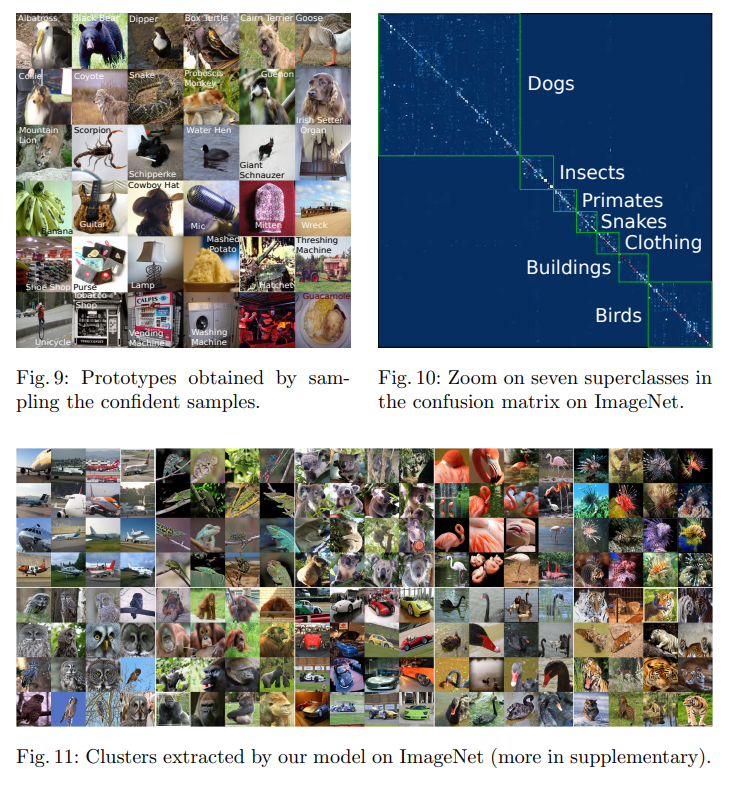
\includegraphics[width=6in]{7.PNG}
\end{center}
\end{figure}
Finally, the table also includes results that compare with the state-of-the-art in representation learning and when solving the problem in a fully-supervised manner. 


\FloatBarrier


\medskip

The Paper considers the problem of unsupervised image classification on the large-scale ImageNet dataset as shown in Table 3. First smaller subsets of 50, 100, and 200 randomly selected classes are considered and then the sets of 50 and 100 classes are subsets of the 100 and 200 classes respectively. 


%%% Imagenet TABLE %%%%
\setlength{\tabcolsep}{4pt}
\begin{table}[ht]
\begin{center}
\caption{Validation set results for 50, 100 and 200 randomly selected classes from ImageNet.}
\label{table: imagenet_subsets}
\resizebox{\columnwidth}{!}{
\begin{tabular}{@{}l c cccc c cccc c cccc@{}}
\toprule
\textbf{ImageNet} && \multicolumn{4}{c}{\textbf{50 Classes}} && \multicolumn{4}{c}{\textbf{100 Classes}} && \multicolumn{4}{c}{\textbf{200 Classes}} \\
\cmidrule{3-6} \cmidrule{8-11} \cmidrule{13-16}
\textbf{Metric} && Top-1 & Top-5 & NMI & ARI && Top-1 & Top-5 & NMI & ARI && Top-1 & Top-5 & NMI & ARI \\
\midrule
\noalign{\smallskip}
\textbf{K-means} && 65.9& - & 77.5 & 57.9 && 59.7 & - & 76.1 & 50.8 && 52.5& - & 75.5& 43.2 \\
\textbf{SCAN$^{*}$} && 75.1 & 91.9 & 80.5 & 63.5 && 66.2 & 88.1 & 78.7 & 54.4 && 56.3 & 80.3 & 75.7 & 44.1 \\
\textbf{SCAN$^{\dagger}$}  && 76.8 & 91.4 & 82.2 & 66.1 && 68.9 & 86.1 & 80.8 & 57.6 && 58.1 & 80.6 & 77.2 & 47.0 \\
\bottomrule
\end{tabular}
}
\end{center}

\end{table}
\setlength{\tabcolsep}{1.4pt}
 

\subsection{Overclustering}  

The network was trained with the knowledge of the number of ground-truth classes. However, the table 2 also reports the results when the number of clusters does not match the number of ground-truth classes. 

It can be observed that the approach does not require knowledge of the exact number of clusters and the increased performance on CIFAR100-20 is related to the higher intra-class variance. 

%\begin{figure}[!htbp]
%\begin{center}
%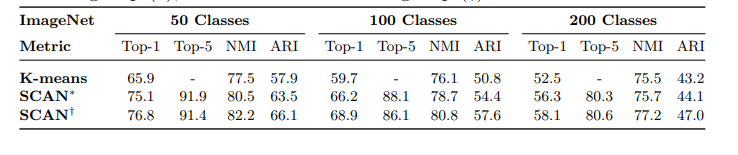
\includegraphics[width=6in]{4.PNG}
%\caption{Overclustering Figure}
%\end{center}
%\end{figure}



